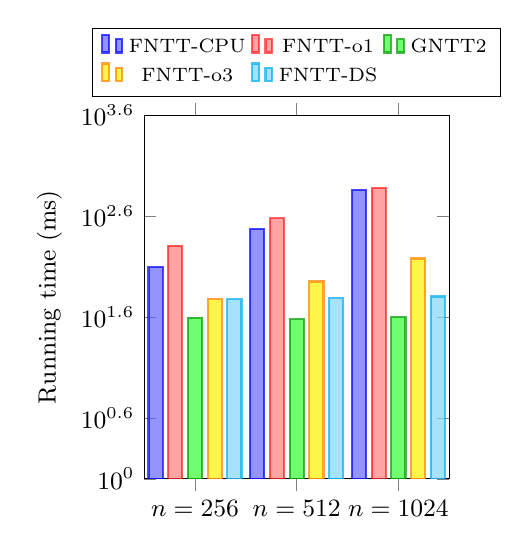
\begin{tikzpicture}
    \begin{axis}[
        ybar, 
        symbolic x coords={$n=256$, $n=512$, $n=1024$},  
        xtick=data,  
        ymode=log,  
        xticklabel style={font=\small},
        yticklabel style={font=\small},
        ylabel={\small Running time (ms)},  
        width=0.45\linewidth,
        height=6.2cm,
        bar width=0.18cm,  
        enlarge x limits=0.25,  
        ymin=1,  
        ymax=4000,
        ytick={1, 4, 40, 400, 4000}, 
        ylabel near ticks,
        legend style={
            at={(0.5,1.05)}, 
            anchor=south,    
            legend columns=3, 
            draw=black,      
            fill=white,      
            font=\scriptsize, 
            legend image post style={scale=0.8} 
        },
    ]

    \addplot[fill=blue!60,draw=blue,thick,opacity=0.7]
     coordinates {($n=256$, 125.413) ($n=512$, 299.832) ($n=1024$, 727.731)};  

    \addplot[fill=red!60,draw=red,thick,opacity=0.6]
     coordinates {($n=256$, 204.177) ($n=512$, 381.066) ($n=1024$, 762.482)};  

    \addplot[fill=green!80,draw=green!60!black,thick,opacity=0.7]
     coordinates {($n=256$, 39.533) ($n=512$, 38.055) ($n=1024$, 40.129)};   

     \addplot[fill=yellow,draw=orange,thick,opacity=0.7]
    coordinates {($n=256$, 60.873) ($n=512$, 90.361) ($n=1024$, 152.783)};  
    
    \addplot[fill=cyan!50,draw=cyan,thick,opacity=0.7]
    coordinates {($n=256$, 60.169) ($n=512$, 61.552) ($n=1024$, 64.263)};

    \legend{FNTT-CPU, FNTT-o1, GNTT2, FNTT-o3, FNTT-DS}

    \end{axis}
\end{tikzpicture}